\section{Operating System Considerations}
\label{os-considerations}
%\subsection{Evolved Embedded Applications}

In a first evolutionary cycle of the embedded devices applications were written
as a essential part of a runtime environment on the device. During secondary
cycle operating systems like TinyOS, Contiki, FreeRTOS emerged separating
application and OS spaces. The development became easier  and applications
got complex but the resulting code was still compiled to a monolithic image and
uploaded to the device.

Now the third evolutionary cycle is emerging: multiple and independently
developed application has to co-exist on the same device (like in Pebble watch);
and embedded devices are becoming modular. The later is evident with
multi-billion companies like Samsung, Telefonica and GE innovating with SimBand, Wzzard, ThinkingThings, Spotter UNIQ.
%~\endnote{http://www.samsung.com/us/globalinnovation/innovation_areas/}, Wzzard
%~\endnote{http://bb-smartsensing.com/wzzard-sensing-platform/}, ThinkingThings
%~\endnote{http://www.thinkingthings.telefonica.com/}, Spotter UNIQ
%~\endnote{https://www.quirky.com/shop/982-spotter-uniq-customizable-multipurpose-sensor}
The aim is to create a core hardware platform where adding sensory
peripherals is done by consumer in a Lego-like fashion while developer compiles
application with provided SDK.

These trends completely change the way applications for the embedded devices
have been developed last five decades. Developer have very little control on the
application execution model, its coexistence with other application and what
peripherals are connected to the embedded device. Instead application developer
expect that underlying operating system will perform fair resource allocation,
protect the application from malicious or malfunctioning applications and
peripherals. 

Given the paradigm shift in embedded devices we design new operating system
\name that supports a combinations of goals:


\begin{itemize}
  \item Event-driven execution model
  \item Loadable applications, services and drivers
  \item Robust, Reliable and Safe %isolation
  \item Energy Efficient 
\end{itemize}



\subsection{Application execution model}
\begin{figure}
 \centering
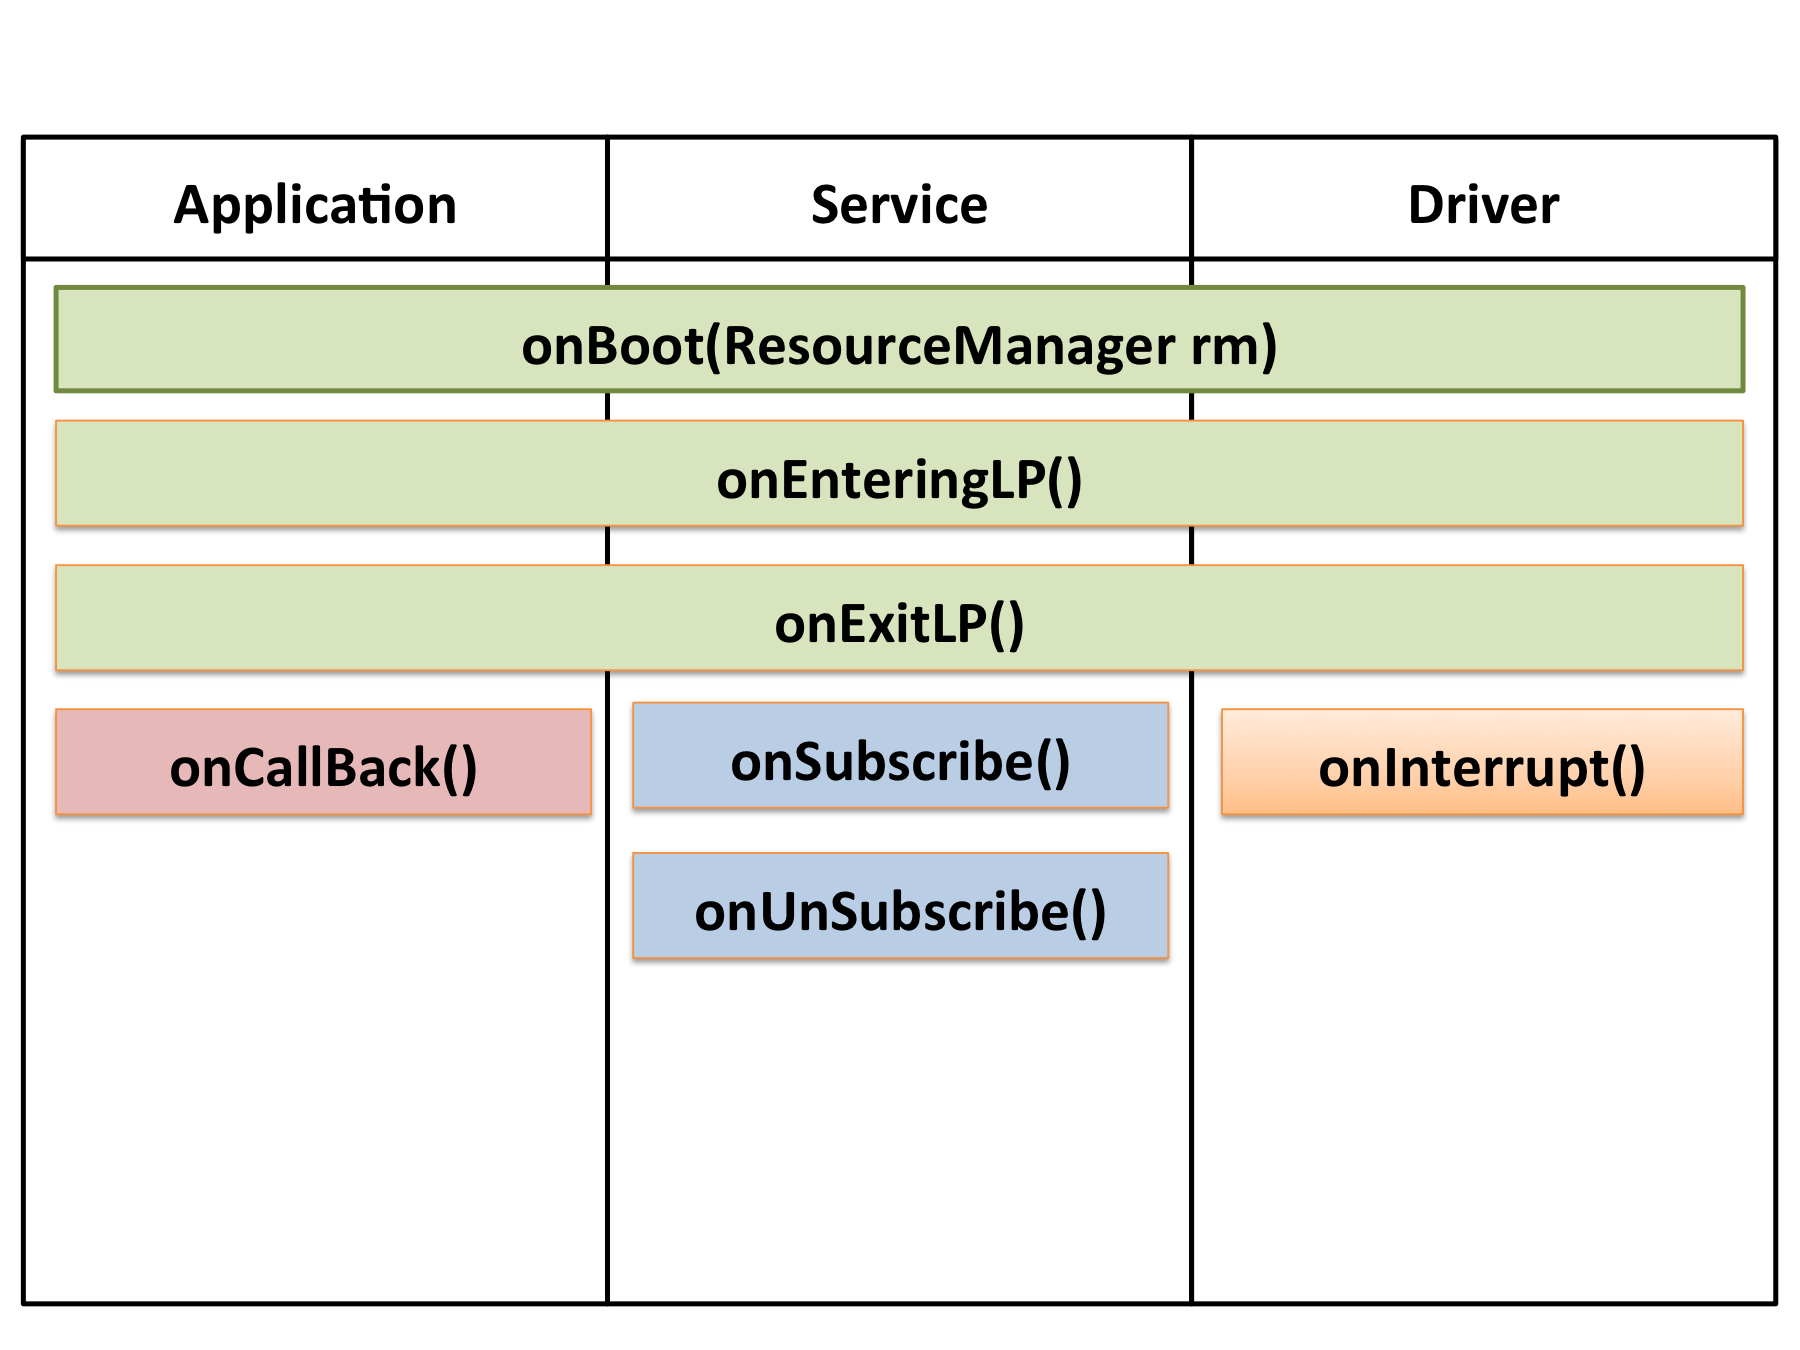
\includegraphics[width=1\columnwidth]{img/appcycle.png}
\caption{Runnable life cycle.}
 \label{fig:appcycle}
\end{figure}


\subsection{Loadable applications, services and drivers}

\name provides a system-call interface. This
allows developers to write applications in any language that can support the
ABI. For example, the \name kernel is written in Rust~\cite{rust}, applications
can trivially written in C, and we are working on a port of Lua~\cite{lua}.

\subsection{Robust, Reliable and Safe}
%tobe rewriten
 \name follows previous operating systems in separating
drivers for core peripherals (SPI, USART, GPIO, etc) and device drivers (radio,
flash, etc) into separate layers. \name differs from previous operating systems
in enforcing safety policies on device drivers through the Rust type system.
\name prevents drivers from subverting Rust's memory safety by restricting
device drivers to a safe subset of the Rust language.~\endnote{Rust allows code
to circumvent the type system using the \tt{unsafe} keyword. \name uses a
compiler flag that disallows this keyword when compiling device drivers.} \name
also ensures, at compile time, that at most one driver has access to a specific
hardware resource---multiplexing must be done explicitly in the core peripheral
driver or through an intermediate interface. Finally, \name ensures device
drivers cannot corrupt kernel memory through careful choice of interfaces. \name
ensures that \name does not protect the kernel from denial of service attacks by
drivers.

{\bf Reliability}. Unlike most desktop and server applications, embedded
applications must continue to run without end-user intervention. There is no
console to indicate to the user that an application has crashed. Even if a crash
could be communicated to the user, there is little action she could take. While
a Blue-Screen-Of-Death is annoying on a desktop or server, it is unacceptable in
embedded systems. Unlike other embedded operating systems, in \name,
applications cannot corrupt the kernel or other applications. Moreover, certain
parts of the kernel (e.g. contributed device drivers) are isolated using
a strong language type system.

\subsection{Energy Efficient}


\subsection{Scheduling}


